\documentclass[12pt,a4paper]{article}
\usepackage[utf8]{inputenc}
\RequirePackage{fix-cm}
\usepackage[english]{babel}
\usepackage{amsmath}
\usepackage{amsfonts}
\usepackage{amssymb, cancel}
\usepackage[table,xcdraw]{xcolor}
\usepackage{graphicx}
\usepackage[left=2cm, right=2cm, top=2.00cm, bottom=2.00cm]{geometry}
\usepackage{setspace}
\usepackage{longtable}
\usepackage{fancyhdr}
\usepackage{cancel}
\usepackage{listings,wrapfig,caption,subcaption}
\usepackage{float}
\usepackage{tikz}
\usepackage{appendix}
\usepackage{lscape}
\usepackage{diagbox}
\usepackage{multirow}
\usepackage{hhline}
\usepackage{enumitem}
\usepackage{verbatim}
\usepackage[breakable]{tcolorbox}
\usepackage{parskip}
\usepackage{hyperref}
\usepackage{cleveref}

% Code styles
\lstdefinestyle{bash}{
  language=bash,
  basicstyle=\ttfamily\small,
  keywordstyle=\color{green!50!black},
  stringstyle=\color{red!60!black},
  commentstyle=\color{gray},
  showstringspaces=false,
  breaklines=true,
  frame=single,
  rulecolor=\color{black!30},
  backgroundcolor=\color{black!5},
  xleftmargin=1em,
  xrightmargin=1em,
}

\newcommand{\bashline}[1]{\lstinline[style=bash]!#1!}

\newcommand{\F}{\textsuperscript{25}F }

\begin{document}

\noindent\rule{\linewidth}{0.6pt}

\begin{center}
    \textbf{\textsf{\Large G249 Anlysis Report}}

    {\textsf{\normalsize \textit{Pablo González Rusell}}}
\end{center}
\noindent\rule{\linewidth}{0.6pt}

\begin{figure}[H]
    \centering
    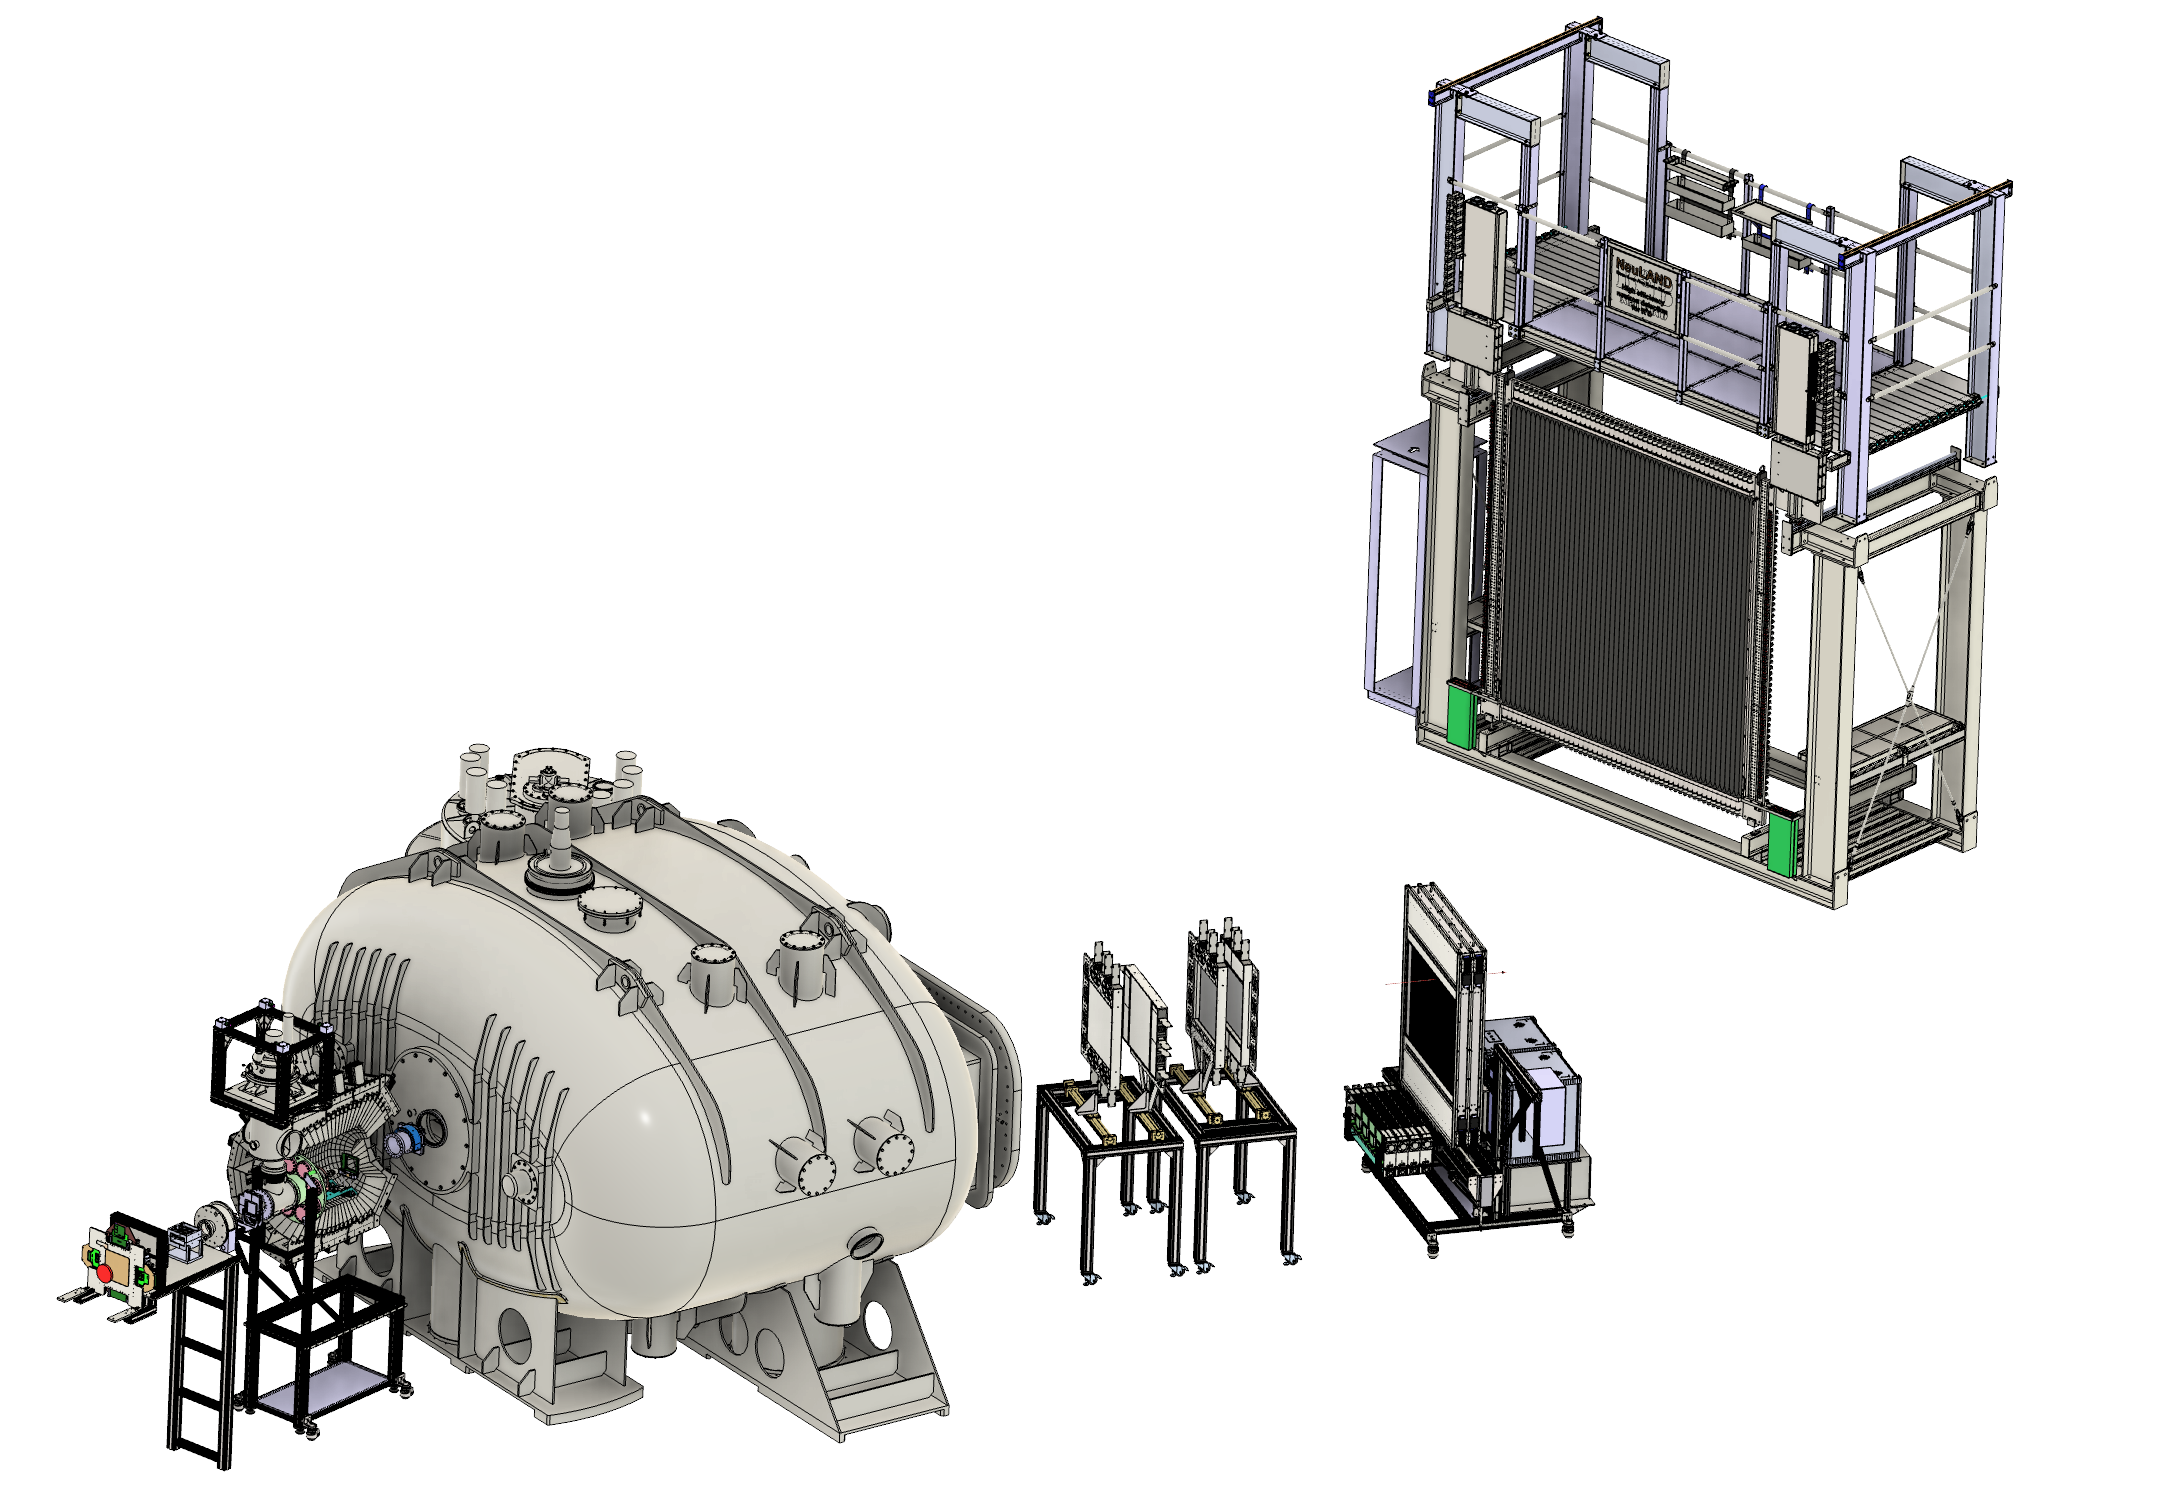
\includegraphics[width=0.6\textwidth]{figures/g249_setup.png}
\end{figure}

This document is a brief description of the different task performed in the analysis of the G249 experiment. In particular we focus on the work done by the macros of the GitHub repository \href{https://github.com/pgrusell/g249_analysis}{g249\_analysis}.


\section{Cross sections}

The first objective is to calculate the cross section for the population of the \textsuperscript{24}O\textsubscript{g.s}, which follows the equation:

$$\sigma = -\frac{M_t}{\rho_tN_Az}\ln\left(1-\frac{N_{frag}^{p2p}}{N_{proj}\epsilon_{p2p}\epsilon_{ToT}\epsilon_{frag}^{rel}}\right)$$

Where:

\begin{itemize}
    \item $M_t$ is the molar mass of the LH\textsubscript{2} target: $M_t=1.000784$ g/mol.
    \item Density of the LH\textsubscript{2} target: $\rho_t = 0.0715$ g/cm\textsuperscript{3}.
    \item Length of the target: $z=5$ cm.
    \item Avogadro's number: $N_A=6.022\times 10^{23}$.
\end{itemize}

\subsection{$N_{proj}$}



$N_{proj}$ represents the number of projectiles that arrive at the target. This number will be calculated from the unreacted beam after the target. This can be done as follows:

$$N_{proj} = \frac{N_{unreacted}}{1 - \text{reaction rate}}$$

Where the reaction rate is given by \href{https://web-docs.gsi.de/~weick/atima/}{ATIMA}. The advantage of this method is that if we count the number of unreacted fragments with the same method as the reacted fragments (MDF, as will be explained later), we don't need to take into account the efficiencies in the detectors before the target.

The reaction rate for an incoming beam of \textsuperscript{25}F impinging onto a $5$ cm LH\textsubscript{2} target is 0.0024. See \cref{xs_atima_file_scheme} for the specific information regarding the materials considered to calculate the reaction rate.

\begin{figure}[H]
    \centering




    \tikzset{every picture/.style={line width=0.75pt}} %set default line width to 0.75pt        

    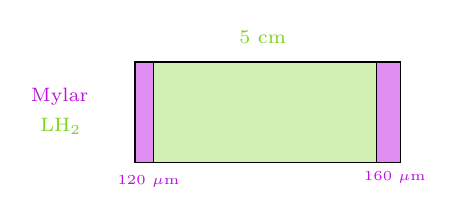
\begin{tikzpicture}[x=0.75pt,y=0.75pt,yscale=-1,xscale=1]
        %uncomment if require: \path (0,217); %set diagram left start at 0, and has height of 217

        %Rounded Same Side Corner Rect [id:dp9107992852496284] 
        \draw  [fill={rgb, 255:red, 126; green, 211; blue, 33 }  ,fill opacity=0.34 ] (422.21,68.72) .. controls (422.21,68.72) and (422.21,68.72) .. (422.21,68.72) -- (422.21,116.99) .. controls (422.21,116.99) and (422.21,116.99) .. (422.21,116.99) -- (314.51,116.99) .. controls (314.51,116.99) and (314.51,116.99) .. (314.51,116.99) -- (314.51,68.72) .. controls (314.51,68.72) and (314.51,68.72) .. (314.51,68.72) -- cycle ;
        %Shape: Rectangle [id:dp6219231022736488] 
        \draw  [fill={rgb, 255:red, 189; green, 16; blue, 224 }  ,fill opacity=0.48 ] (305.75,68.72) -- (314.51,68.72) -- (314.51,117.12) -- (305.75,117.12) -- cycle ;
        %Shape: Rectangle [id:dp1722758653798474] 
        \draw  [fill={rgb, 255:red, 189; green, 16; blue, 224 }  ,fill opacity=0.48 ] (422.21,68.72) -- (433.63,68.72) -- (433.63,117.12) -- (422.21,117.12) -- cycle ;

        % Text Node
        \draw (254.33,80.07) node [anchor=north west][inner sep=0.75pt]  [font=\scriptsize,color={rgb, 255:red, 189; green, 16; blue, 224 }  ,opacity=1 ] [align=left] {Mylar};
        % Text Node
        \draw (258.93,94.61) node [anchor=north west][inner sep=0.75pt]  [font=\scriptsize,color={rgb, 255:red, 126; green, 211; blue, 33 }  ,opacity=1 ] [align=left] {LH$\displaystyle _{\text{2}}$};
        % Text Node
        \draw (296.11,122.25) node [anchor=north west][inner sep=0.75pt]  [color={rgb, 255:red, 189; green, 16; blue, 224 }  ,opacity=1 ] [align=left] {{\tiny 120 $\displaystyle \mu $m}};
        % Text Node
        \draw (354.82,52.44) node [anchor=north west][inner sep=0.75pt]  [font=\scriptsize,color={rgb, 255:red, 126; green, 211; blue, 33 }  ,opacity=1 ] [align=left] {5 cm};
        % Text Node
        \draw (414.81,120.23) node [anchor=north west][inner sep=0.75pt]  [color={rgb, 255:red, 189; green, 16; blue, 224 }  ,opacity=1 ] [align=left] {{\tiny 160 $\displaystyle \mu $m}};

    \end{tikzpicture}


    \caption{Scheme of the materials used in the ATIMA file to calculate the reaction rate}
    \label{xs_atima_file_scheme}
\end{figure}

\subsubsection{Incoming selection}

Now we have the reaction rate, the following step is to count the number of \F that didn't react. The first condition that we are going to apply is the selection of the \F as incoming in the FRS/LOS setting. To do this, we apply a rectangular cut in the A/Q (from FRS data) vs Z (from LOS data) plot in the region of the \F. The values used are: $8.2 \leq Z \leq 10$ and $2.77 \leq A/Q \leq 2.79$. The result of the cut is shown in the following figure:

\begin{figure}[H]

    \centering
    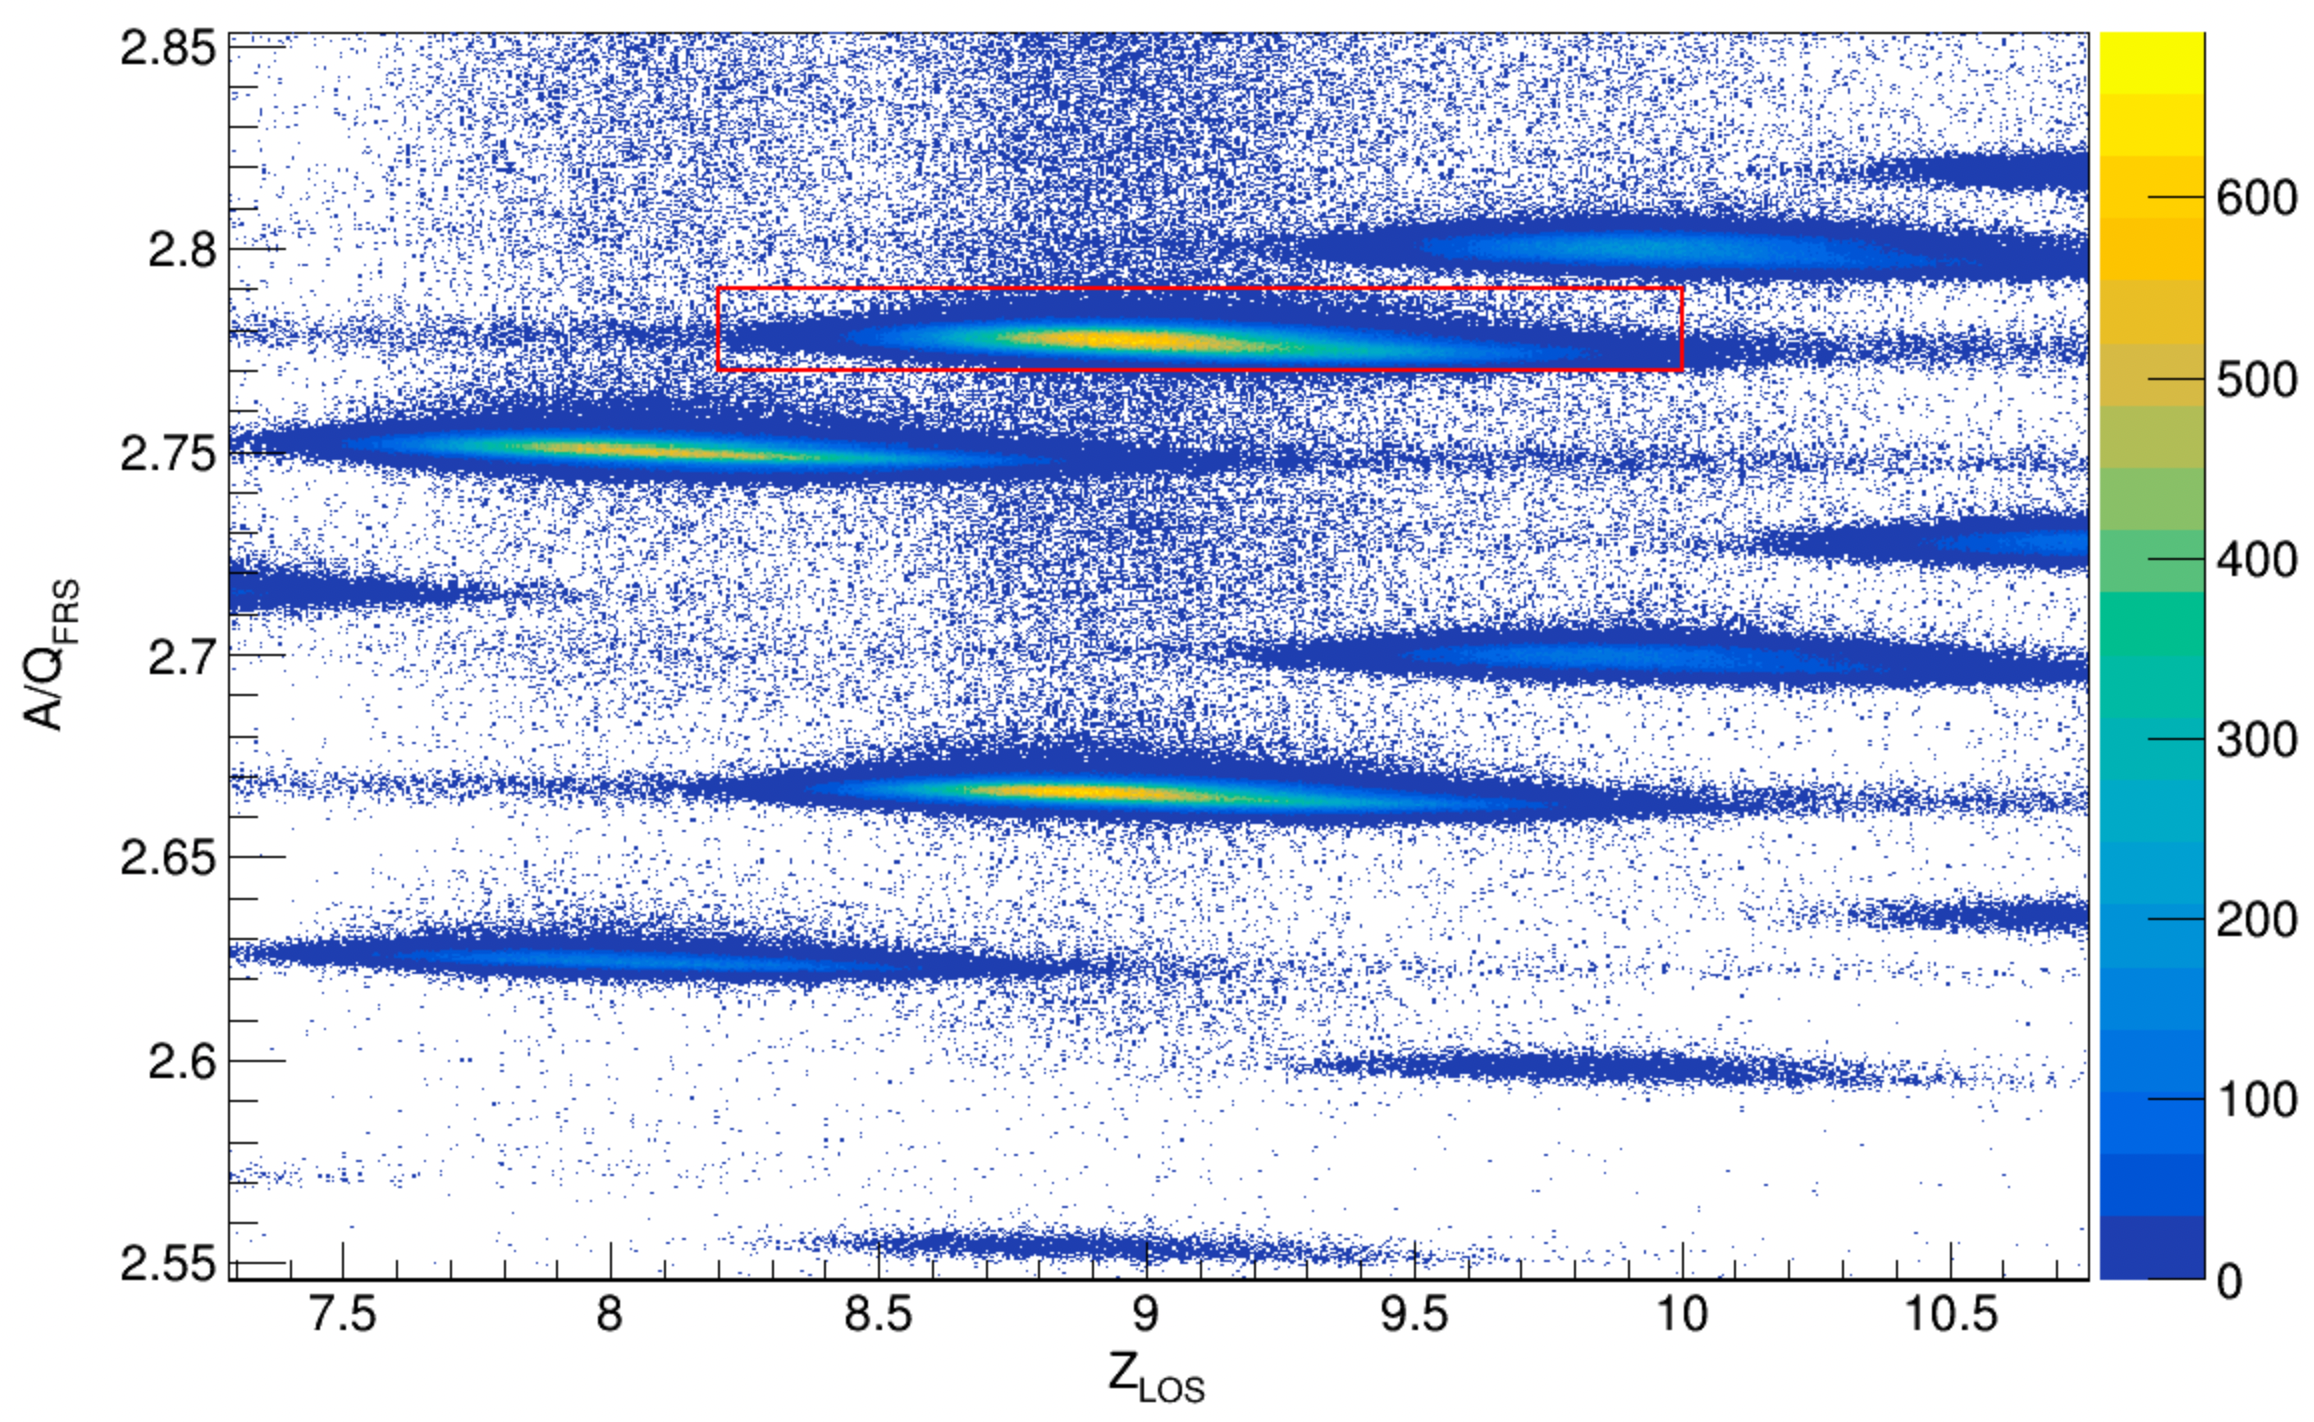
\includegraphics[width=0.6\textwidth]{figures/xs_aoq_vs_Z_cut_incoming.png}
    \caption{A/Q from FRS vs Z from LOS to make the identification of the incoming beam. In red, cut applied to select just \F.}
\end{figure}

The first thing that we notice here is that a better way to select the incoming is clearly needed as this seems not to be the best way possible. Nevertheless, the effect is probably not so big, since it should affect in the same way to the number of projectiles reconstructed from the unreacted and the \textsuperscript{24}O measured, but it's anyway a source of systematic uncertainties.

\subsubsection{Unreacted selection: MDF}

After applying this cut, we will look for the \F that did not react after the target in the MDF. This MDF, have the following restrictions:

\begin{enumerate}
    \item Data (the branch itself) of the following detectors has to be present: LOS, FRS (both within some AoQ/Z cut), IncomingFootTrack and OutgoingFootTrack, FootHitData (which is redundant since the outgoing/incoming tracks are reconstructed from it), TofdHitData and Fiber data.

    \item Certain parameters such as glad current, FrsCutMeanZ... have to be set in the macro of the unpacker.

    \item For an event to be considered, it has to have information of FRS, LOS, first plane of ToFD (within a given energy window), foot\_incoming, foot\_outgoing, fib30 (X) and fib32 (Y).

    \item At least one of the fibers 31 and 33 have to have data (since they share plane).

    \item In order to make the tracking (incoming and outgoing) of the FOOTs, following conditions are necessary:

          \begin{itemize}
              \item FootHitData and FRSData.
              \item Just 8 FOOTs in the mapping parameters.
              \item The VFTX number in the FRS data has to be the same as selected\footnote{This is due to the fact that during our experiment a second VFTX was installed in the middle of the beam time. Since it has better resolution and acceptance it is the one that we should use when available.}.
              \item Only the highest energy hit in every detector will be used.
              \item Data in all 8 FOOTs has to be present.
          \end{itemize}

    \item For fibers, only the highest energy hit in every fiber will be used for this reconstruction. In case that there is signal both in Fib31 and Fib33 the one with higher energy will be used.
\end{enumerate}

Under these conditions, the MDF provide information regarding the A/Q and P/Q of the outgoing fragment after the target that, together with the charge in ToFD, will make possible the outgoing frgament identification.

In the first case of interest, we will select the unreacted \F, from the A/Q vs Z plot. As we can see, the unreacted clearly dominates over the rest of the isotopes. As first approximation, we can consider that, for a sufficiently narrow cut around the centroid of the \F ``blop'', the contamination from other isotopes is negligible.

\begin{figure}[H]

    \centering
    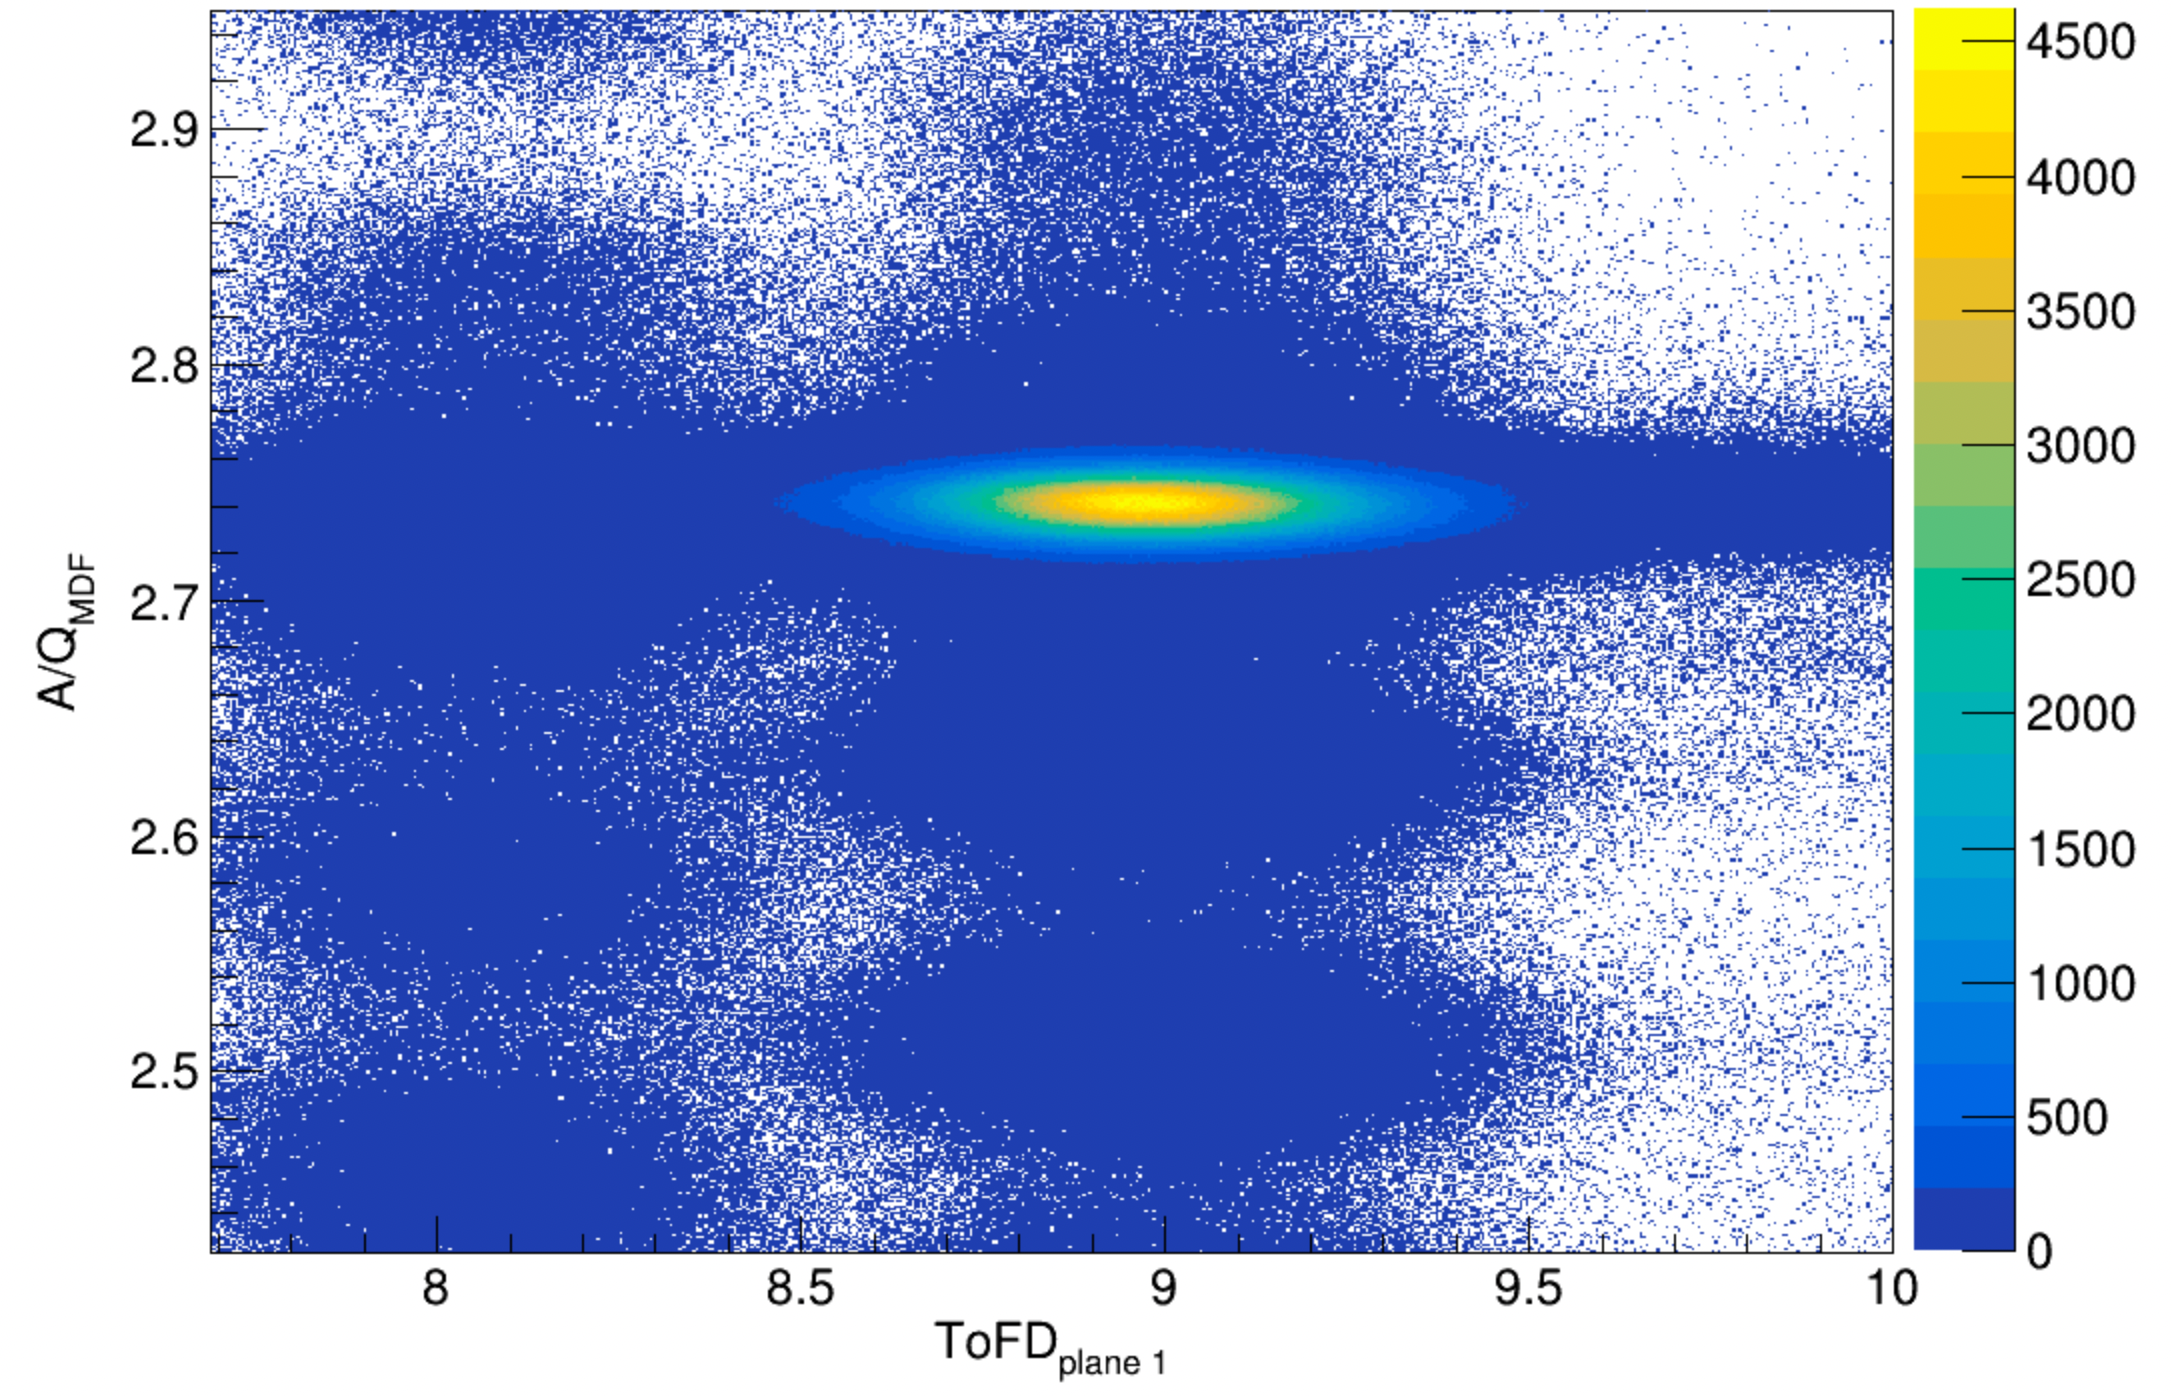
\includegraphics[width=0.6\textwidth]{figures/xs_AoQ_Z_outgoing_25F.png}
    \caption{A/Q (from the MDF) vs Z (from ToFD first plane) with the selection in \F as incoming.}

\end{figure}

In these conditions, to make a systematic selection of the \F we can make a fit to a 2D-Gaussian function:

\begin{equation}
    f(Z, AoQ) = p_0\exp\left[-\frac{1}{2}\left(\frac{Z-p_1}{p_2}\right)^2-\frac{1}{2}\left(\frac{AoQ-p_3}{p_4}\right)^2\right]
\end{equation}

This will provide both centroids of the ``blop'' ($\mu_{AoQ}=2.740$, $\mu_{Z}=8.976$) and the standard deviations ($\sigma_{AoQ} = 0.00988$, $\sigma_{Z}=0.1973$). Thus, a elliptical cut defined in terms of constant number ($k$) of $\sigma$ around the centroid, can be used to select the \F.

Now that we have defined the cut, is important to notice that just counting the number of nuclei inside the cut will bias the result: a higher $k$ will increase the number of isotopes and a smaller cut will reduce it. Hence, is important no estimate the efficiency ($\varepsilon$) of the cut: How many of the real events are inside the cut. One approach could be use the analytical formula of the Gaussian efficiency:

\begin{equation}
    \varepsilon = 1 - e^{-k^2/2}
    \label{gaussian_eff}
\end{equation}

The problem is that the previous fit has a non-negligible background that makes the value of the number of isotopes too unstable.

To avoid this problem we will first select all valid AoQ values, by applying the elliptical in the A/Q vs Z plot. After that, we can histogram all these values, clearly seeing a Gaussian-like behavior. Making a fit to a Gaussian function plus a linear background (see \cref{figs:xs_incoming_estimate_from_fit} left) we can estimate the real number of fragments in the elliptical cut by correcting from contamination (the linear background), and then use \cref{gaussian_eff} to extrapolate and make it independent on the $k$. In \cref{figs:xs_incoming_estimate_from_fit} right, we see that the total variation of the number of isotopes for a window inside of $k\in[3, 4]$ is around $\pm 0.3\%$.

\begin{figure}[htbp]
    \centering
    \begin{subfigure}[b]{0.48\textwidth}
        \centering
        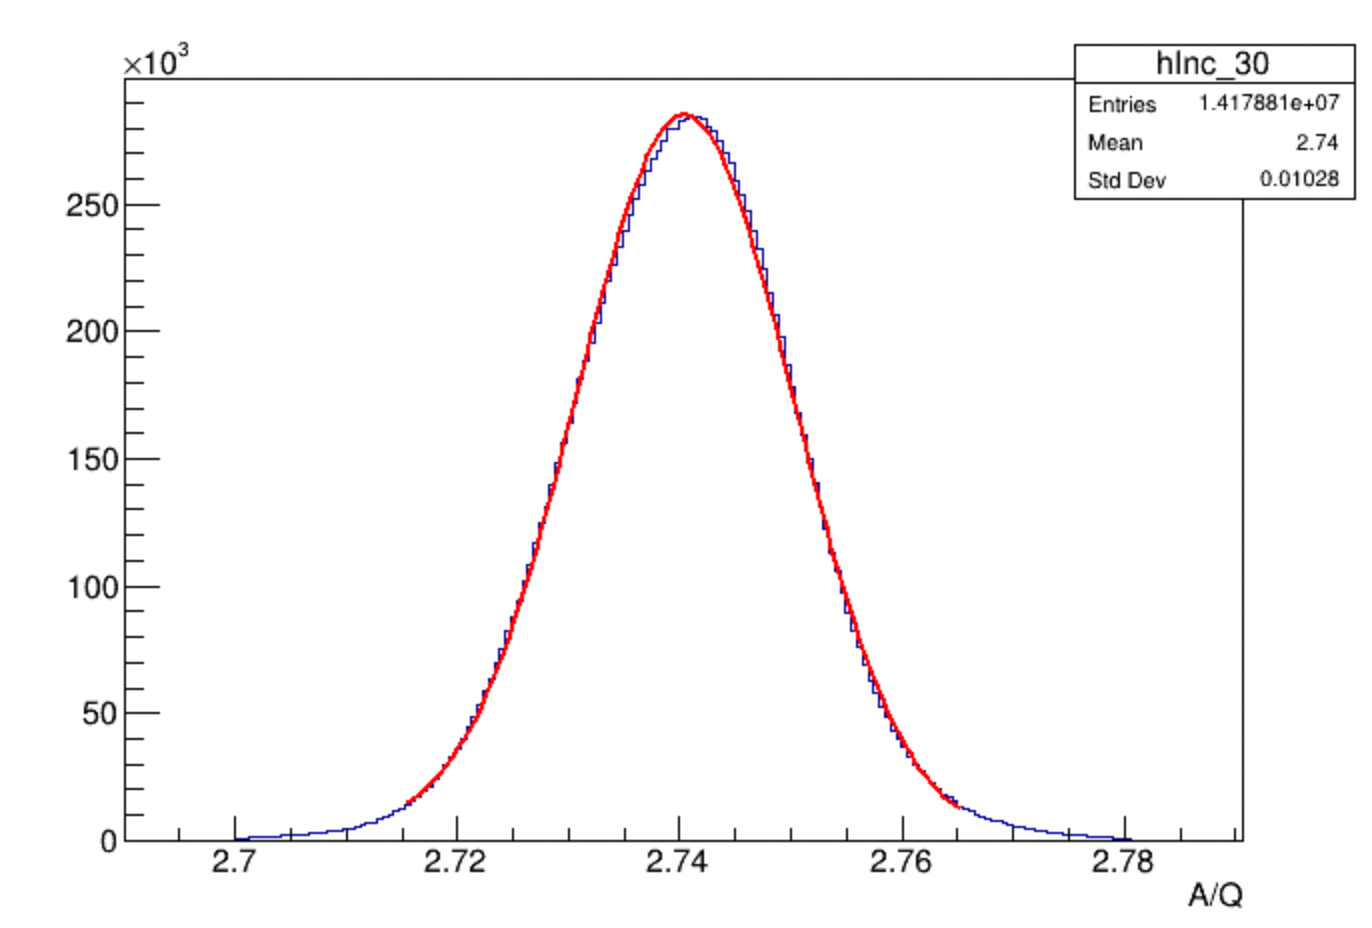
\includegraphics[width=\textwidth]{figures/xs_gaussian_fit_aoq_slices.png}
    \end{subfigure}
    \hfill
    \begin{subfigure}[b]{0.48\textwidth}
        \centering
        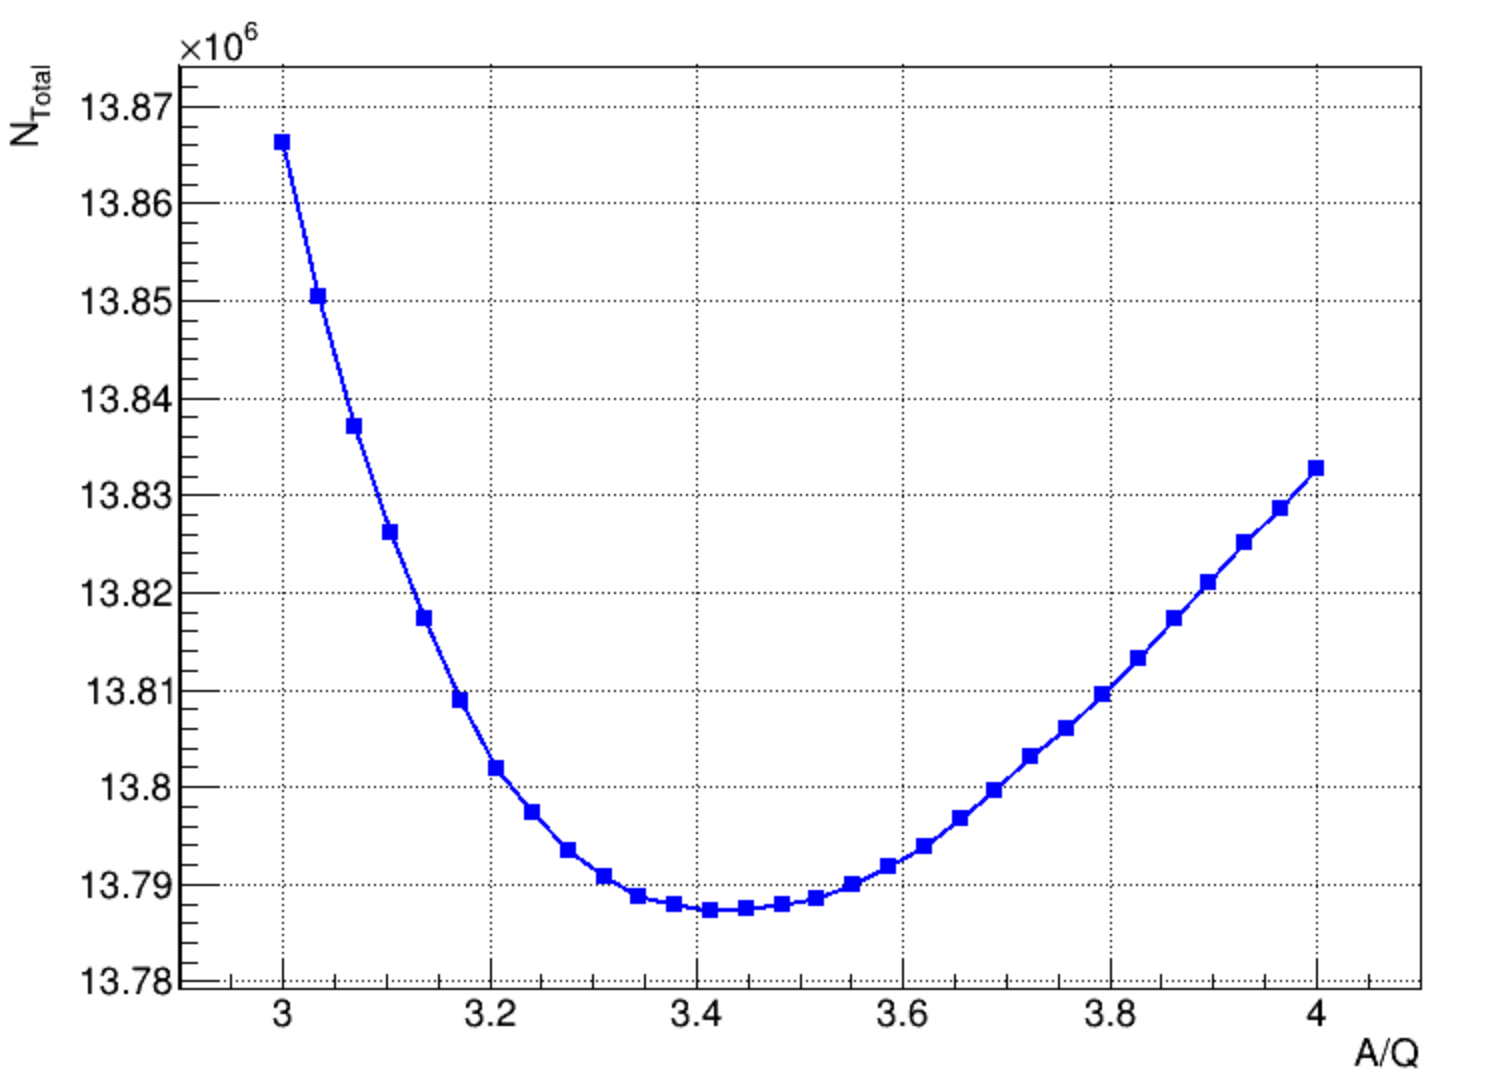
\includegraphics[width=0.9\textwidth]{figures/xs_eff_vs_k.png}
    \end{subfigure}

    \caption{Left: Result of histogramming all AoQs within a $k = 4$ elliptical cut, in blue. Result of the fit to a Gaussian plus linear background, in red. Right: Number of isotopes after efficiency correction as a function of $k$.}
    \label{figs:xs_incoming_estimate_from_fit}
\end{figure}

\subsection{$N_{frag}^{p2p}$}

Once the number of projectiles has been calculated, the next step is to estimate the total amount of \textsuperscript{24}O measured. Since this nucleus does not have any bound states all \textsuperscript{24}O measured will correspond to the population of the ground state. However, to assert that all of them are produced through QFS p2p, we need to look at the opening angle in CALIFA.

In p2p QFS reactions the interaction is considered as elastic scattering between the proton of the target and the valence proton of the \F. After some kinematical calculations the results is that the opening angle between the outgoing protons has to be centered at $82^\circ$.

This information can be used as a kinematical signature of out p2p reactions, before making any cut in the MDF we will ask for additional conditions. In particular:

\begin{itemize}
    \item Two clusters in CALIFA with energies higher that 20 MeV. The selection of this value is motivated by simulations.
    \item These two clusters have to be coplanar. This means that its $\phi$ coordinate should be almost complementary ($\phi_1 + \phi_2 = 180^\circ \pm 30^\circ$).
\end{itemize}

After applying these two conditions (p2p), we can have a look at the number of \textsuperscript{24}O in the A/Q vs Z plot of the MDF. As we see in \cref{xs_24o_pid}, the blops are better separated than in the unreacted case, so no further correction by contamination will be applied.

\begin{figure}[H]
    \centering
    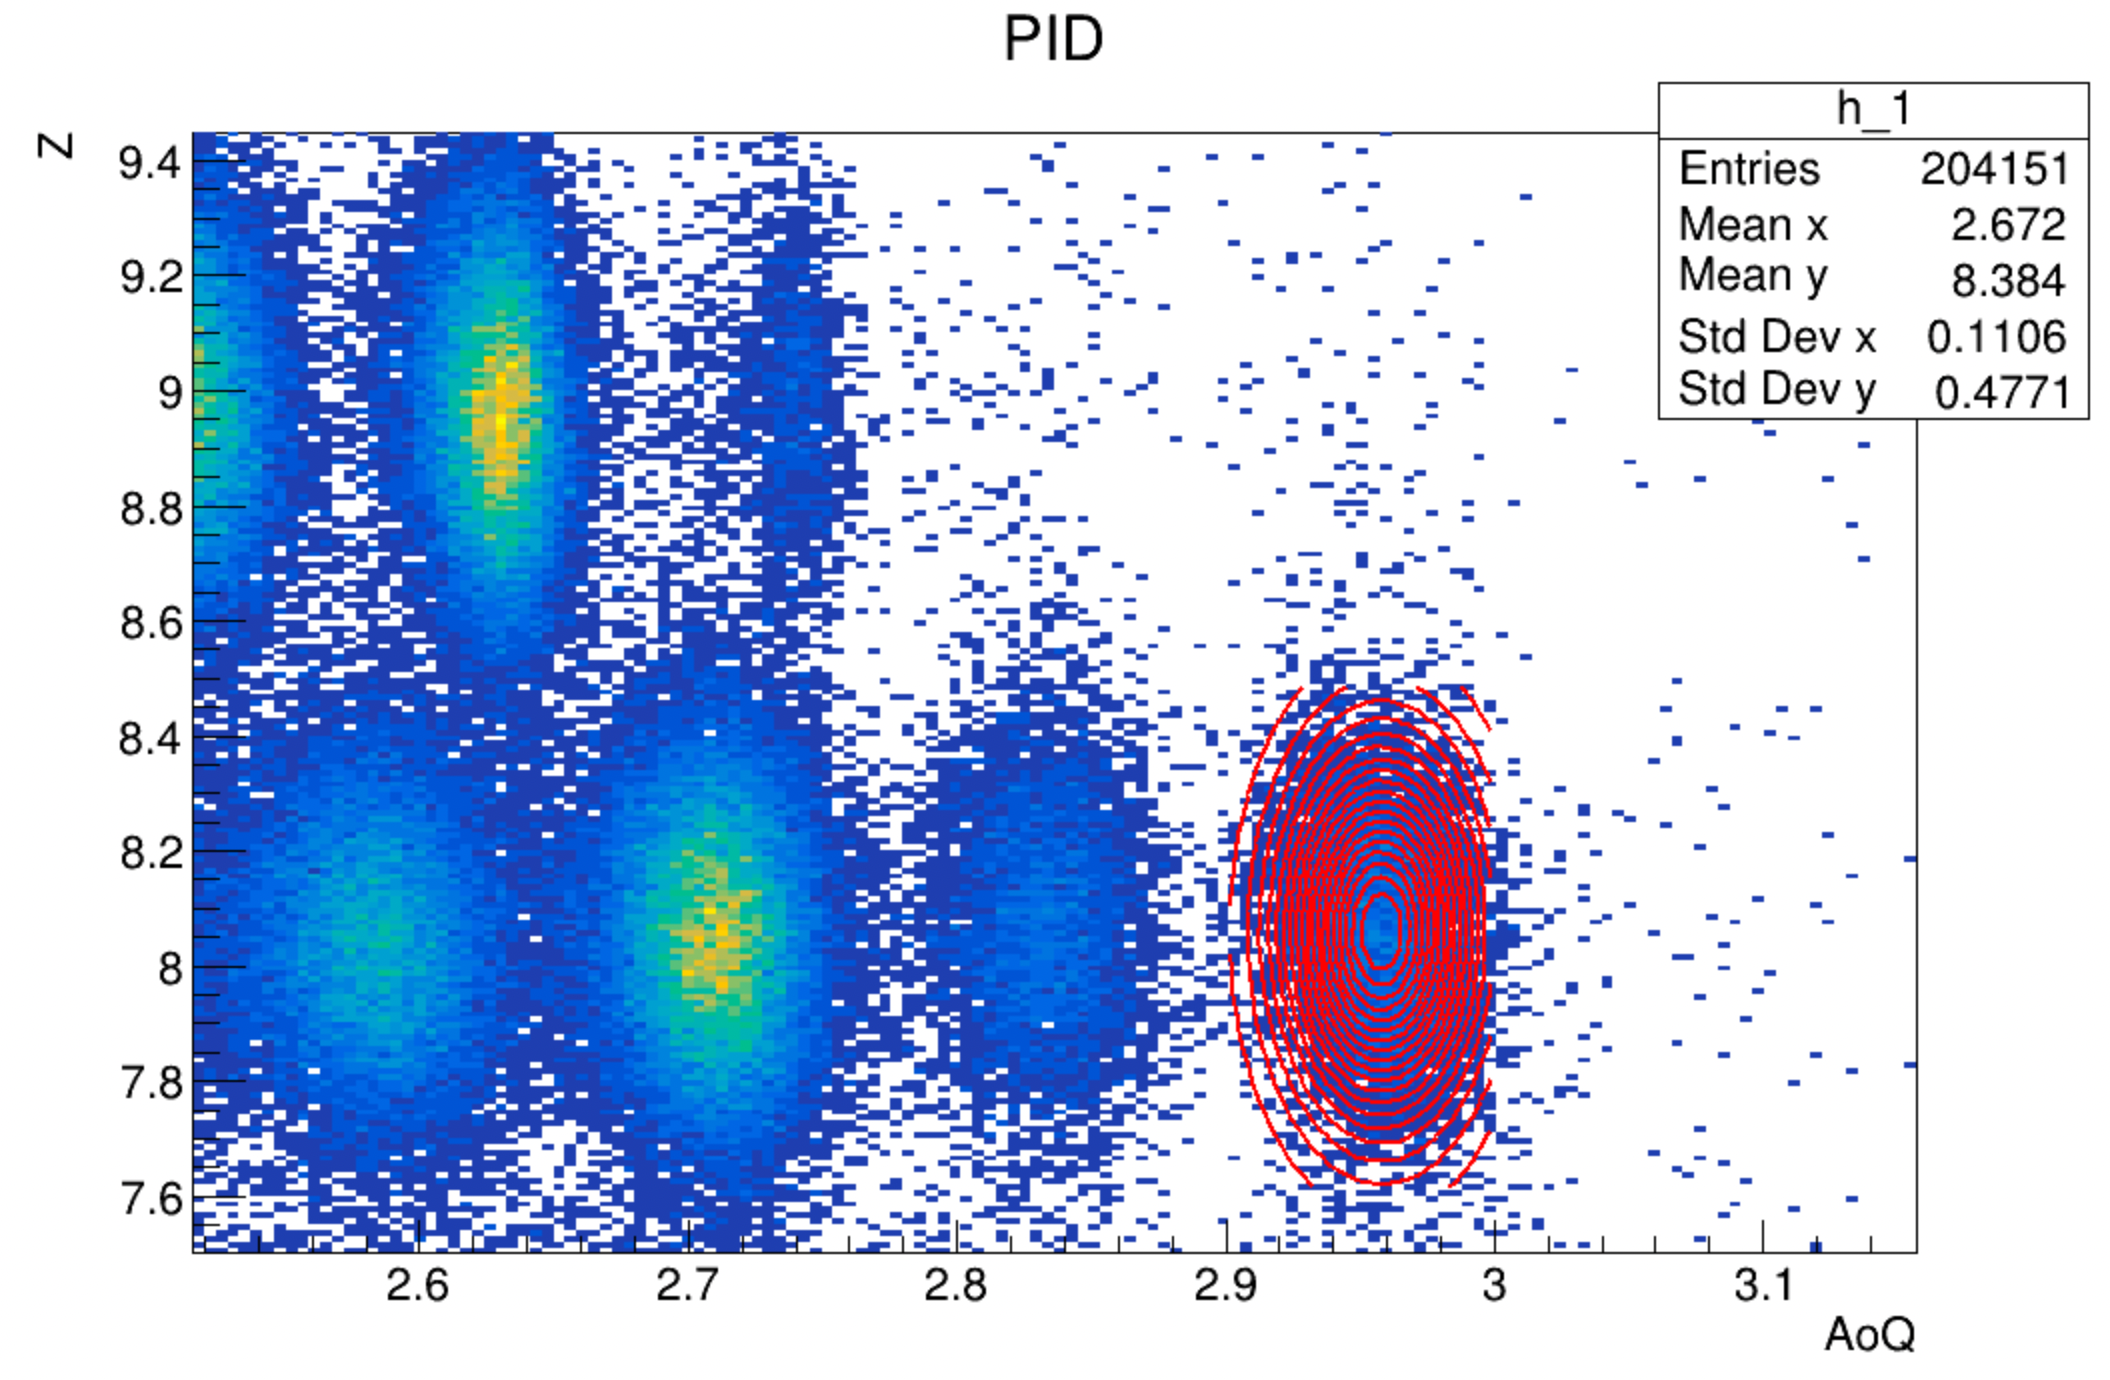
\includegraphics[width=0.8\textwidth]{figures/xs_24o_pid.png}
    \label{xs_24o_pid}
    \caption{A/Q vs Z plot from the MDF with p2p conditions. In red, fit to the \textsuperscript{24}O to a 2D-Gaussian \cref{gaussian_eff}.}
\end{figure}

The next step is to select QFS events, i.e., events that have an opening angle in CALIFA close to the $\sim 82^\circ$. To do this, we can make a Gaussian fit to the QFS peak plus a quadratic background and, again, for a given $k_{\text{opa}}$-value, obtain the number of real p2p-QFS events by correcting the ROI-events by both efficiency and contamination. See \cref{xs_opa_fit}.


\begin{figure}[H]
    \centering
    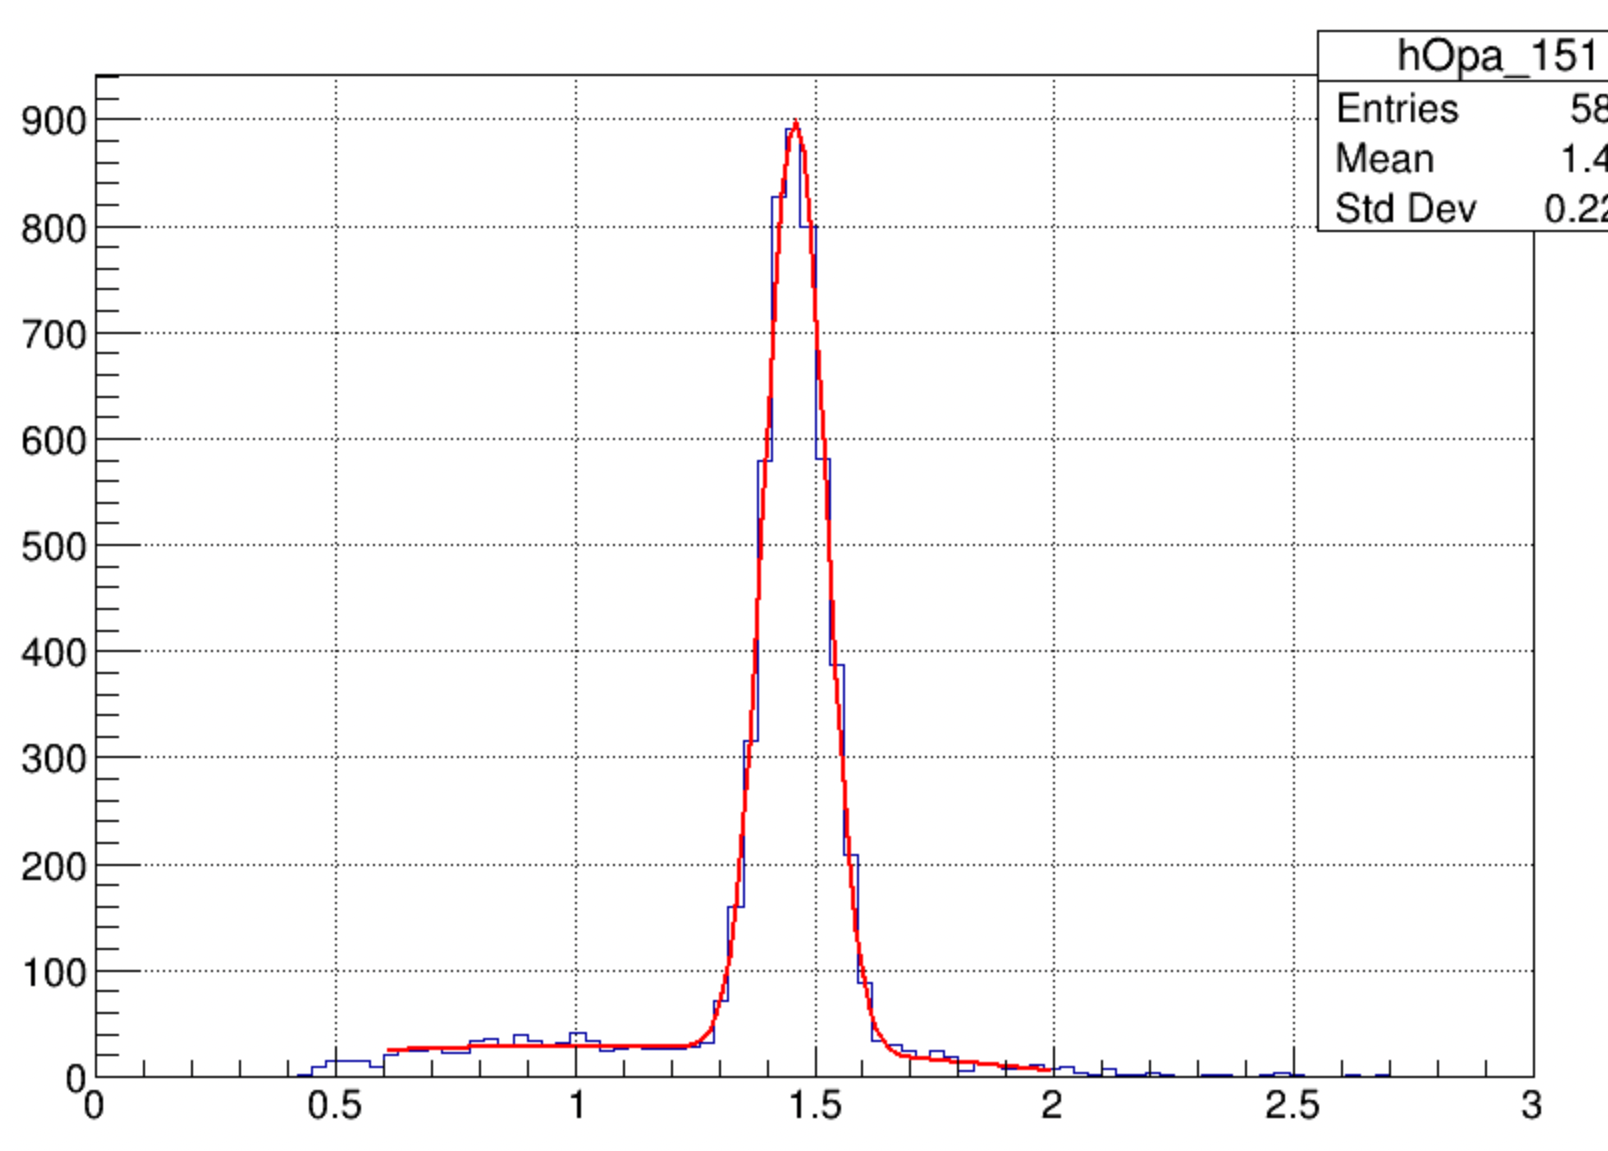
\includegraphics[width=0.7\textwidth]{figures/xs_fit_opa_gaussian.png}
    \label{xs_opa_fit}
    \caption{Fit of the opening angle distribution in CALIFA, after p2p conditions applied and \textsuperscript{24}O selection in MDF using the previous elliptical cut.}
\end{figure}

Regarding stability of both cuts with respect to the parameter $k$ and $k_{\text{opa}}$, we can study the number of fragments as a function of $k$ and $k_{\text{opa}}$. In \cref{figs:xs_out_stabilities} we see that, basically for both $k$ and $k_\text{opa}$, there is a \textit{plateau} where number of fragments is relatively stable.

\begin{figure}[htbp]
    \centering
    \begin{subfigure}[b]{0.48\textwidth}
        \centering
        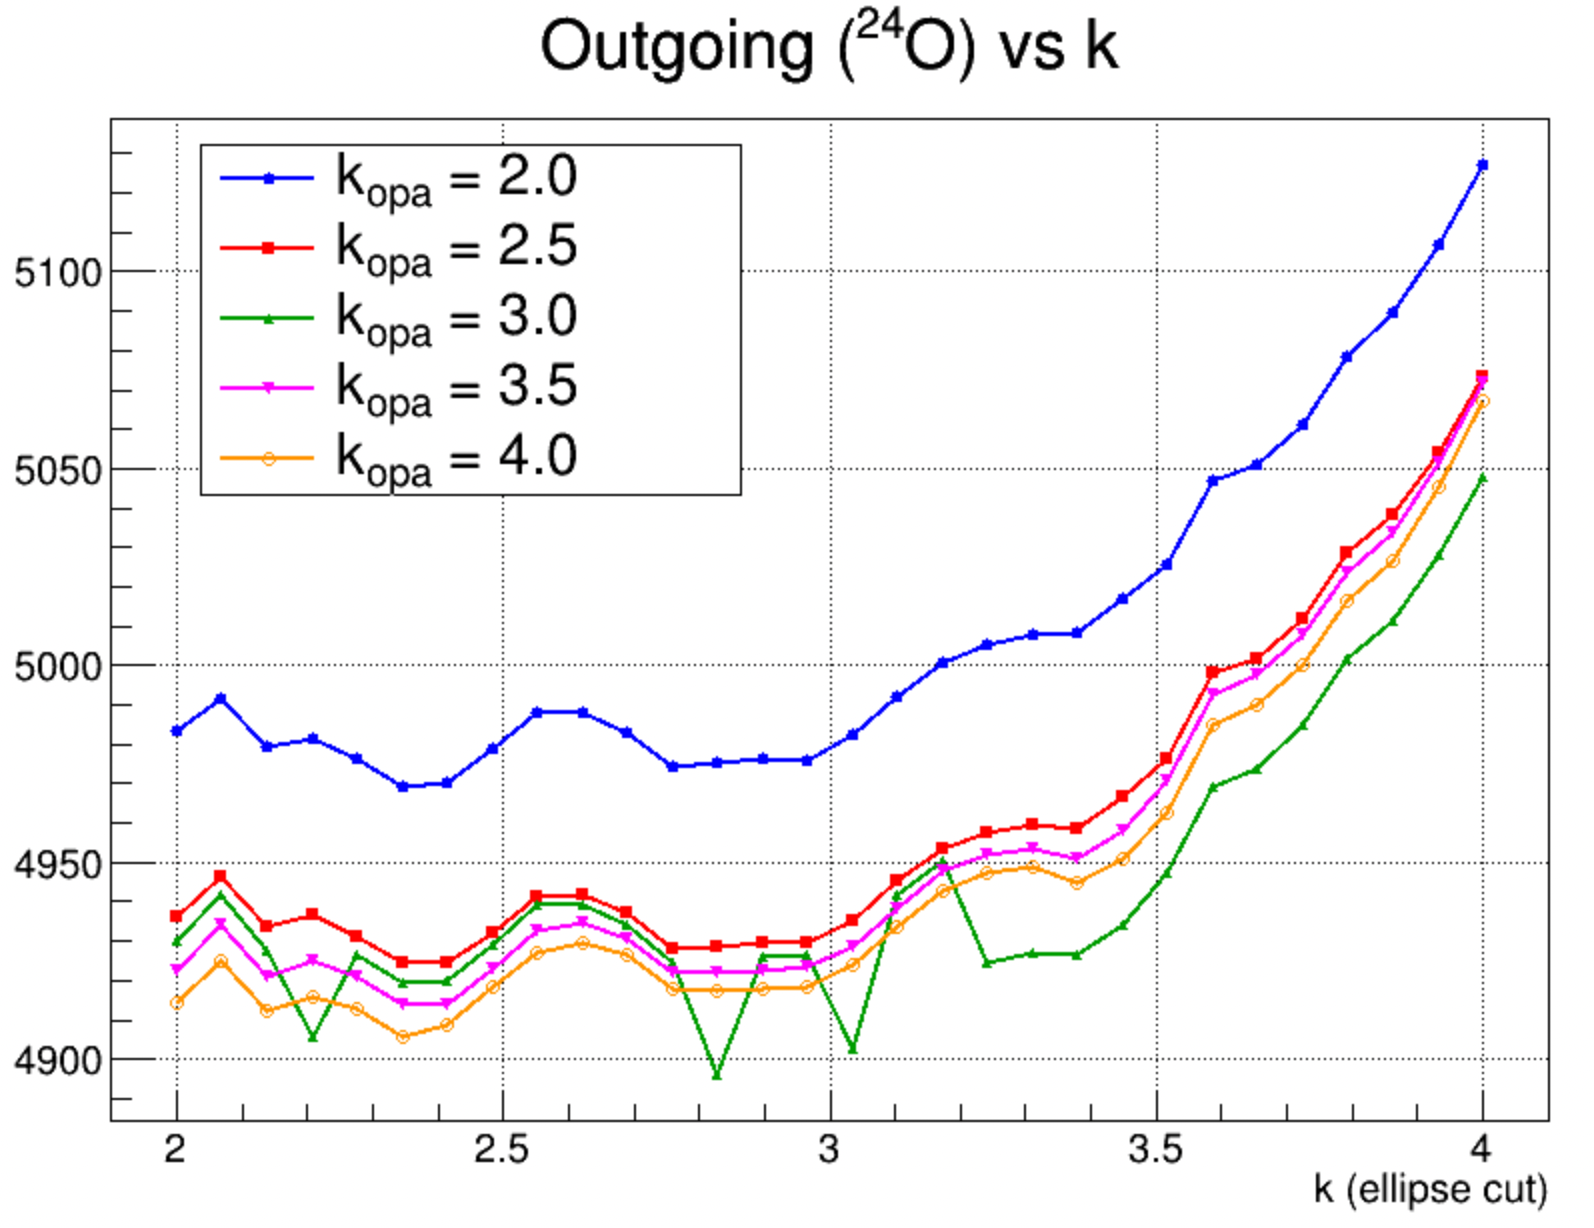
\includegraphics[width=\textwidth]{figures/xs_kcut_vs_yields_manyopas.png}
    \end{subfigure}
    \hfill
    \begin{subfigure}[b]{0.48\textwidth}
        \centering
        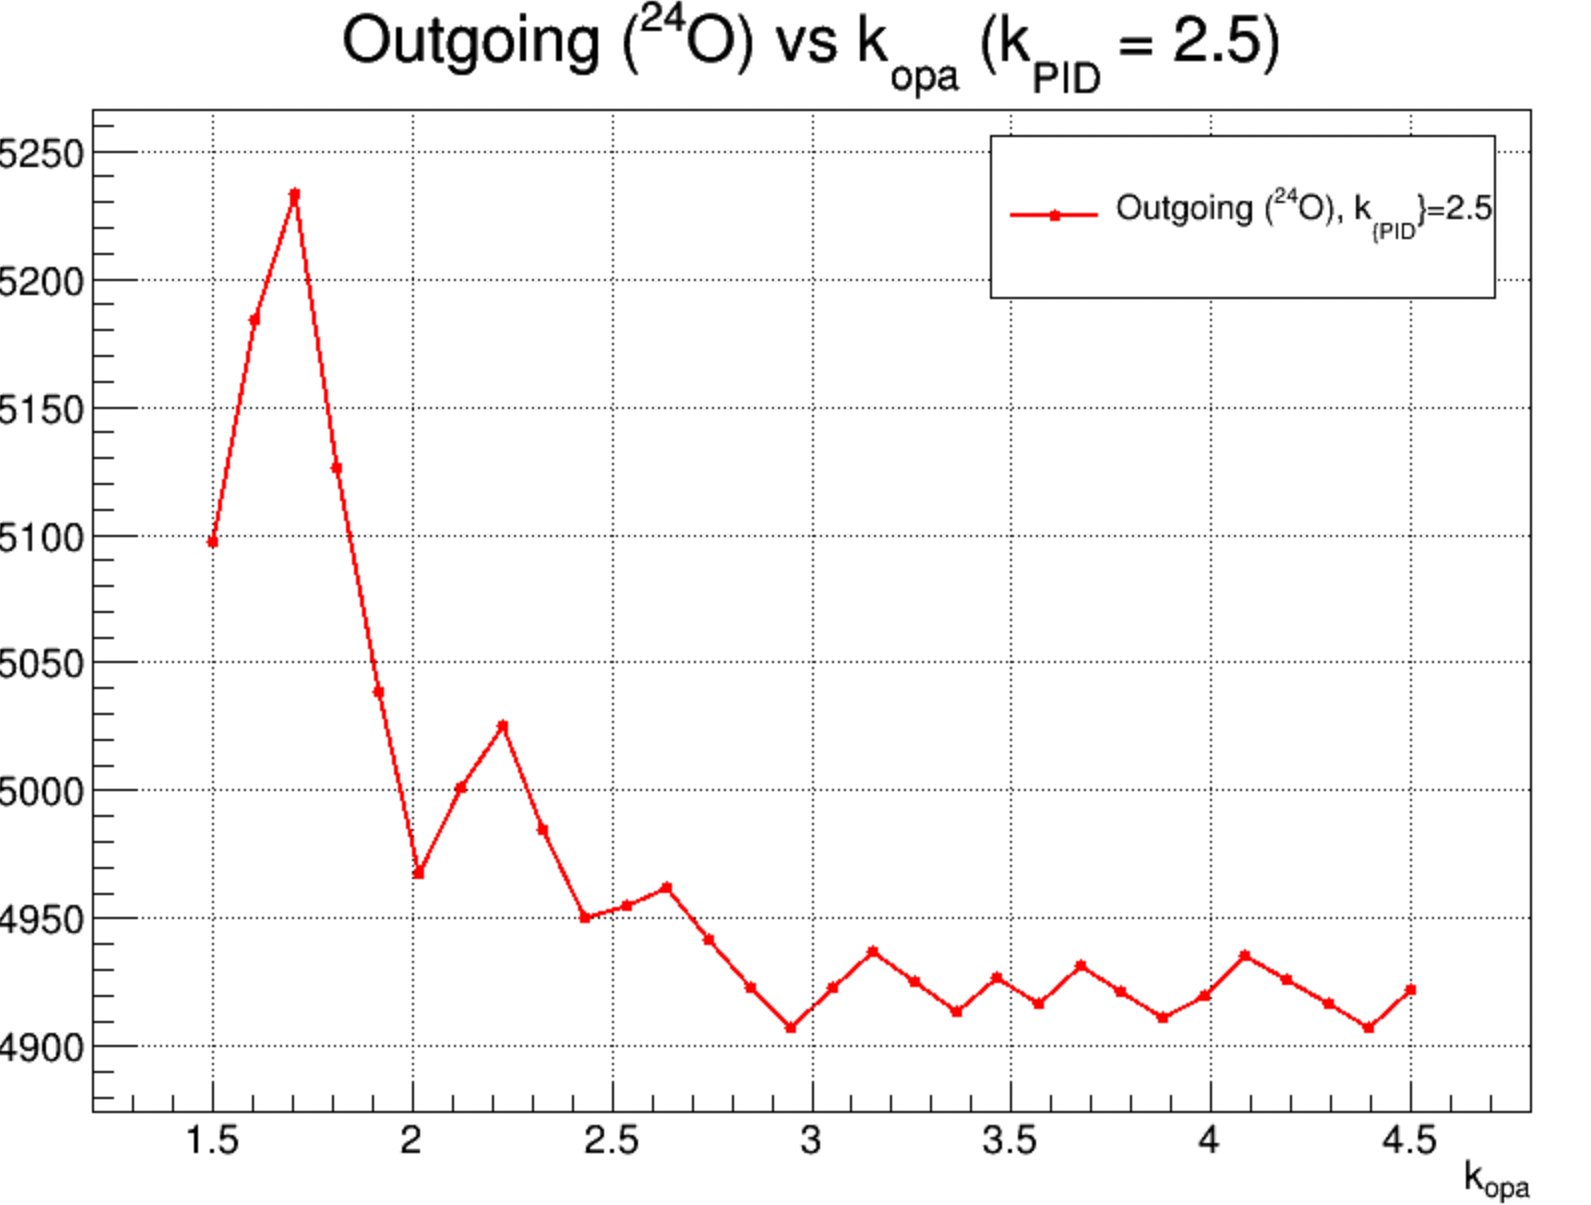
\includegraphics[width=\textwidth]{figures/xs_kopa_vs_yields.png}
    \end{subfigure}

    \caption{Left: Number of fragments as a function of the $k$ value of the elliptical cut for different values of the $k_{\text{opa}}$. Right: Number of fragments as a function of the $k_{\text{opa}}$, for a fixed values of the $k=2.5$ (around the \textit{plateau} region).}
    \label{figs:xs_out_stabilities}
\end{figure}

\subsection{$\epsilon_{p2p}$}

Now that we have the raw number for the number of projectiles and the number of \textsuperscript{24}O produced in the target, it's time to account the possible unefficiencies. It's interesting to note that, since we are calculating a ratio between two quantities, all the uncertainties that affect in the same way the number of projectiles and the number of reactions will cancel out, so we are only interested in the differences between the behaviors of these two isotopes.

The first and more clear difference is that we are using the fact that all p2p reactions will leave a clear signal in CALIFA in form of two high-energy cluster. Nonetheless, this is not true, some protons can escape CALIFA, or have much bigger, or smaller, angle than expected...

This unefficiency has to be taken into account by simulating the response of CALIFA to p2p events generated with INCL.

Concerning CALIFA geometry, we have used the 2025 version with a global offset between CALIFA and the target of -5 cm. This was fine-tunned so the QFS peaks matched the theoretical $\sim 82^{\circ}$ value. Notice that this value can introduce changes in this p2p efficiency, and its effect will be studied later.

\bibliographystyle{plain}
\bibliography{bibliography}




\end{document}
